\documentclass[aspectratio=169,9pt]{beamer}
\usetheme{Madrid}
\usecolortheme{beaver}
\usepackage{graphicx}
\usepackage{booktabs}
\usepackage{colortbl}
\usepackage{amsmath}
\usepackage{xcolor}
\usepackage{inputenc}
\usepackage{tikz}

\definecolor{rowbest}{rgb}{0.82,0.94,0.82}
\definecolor{rownew} {rgb}{0.80,0.90,1.00}
\definecolor{bluecol}{rgb}{0.18,0.42,0.72}

\newcommand{\plots}{figs}
\newcommand{\sE}{\sigma_{\rm END}}
\newcommand{\sT}{\sigma_{\rm TOP}}
\newcommand{\sB}{\sigma_{\rm BLUE}}

%% Verified numbers
\newcommand{\SIGBLUE}{15.21}
\newcommand{\SIGTOP}{15.20}
\newcommand{\SIGEND}{53.68}
\newcommand{\WTOP}{0.987}
\newcommand{\WEND}{0.013}

\title[EndSparseTop: 15\,ps]{From 50\,ps to 15\,ps: EndSparseTop Readout}
\subtitle{How it works, why it works, and what the data say}
\author{Simulation analysis}
\date{2026-08-17 — verified reanalysis}

\begin{document}

% ── 1. HEADLINE ───────────────────────────────────────────────────────────────
\begin{frame}{EndSparseTop: 15\,ps timing with 20 sparse TOP SiPMs}
\begin{columns}[T]
\begin{column}{0.46\textwidth}
\vspace{0.3em}
\begin{center}
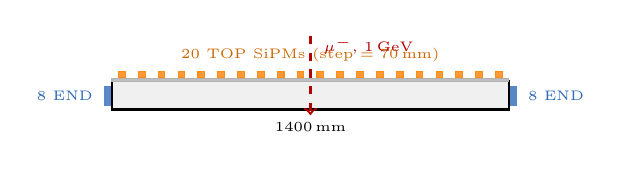
\begin{tikzpicture}[scale=0.60, every node/.style={font=\tiny}]
  \draw[thick,fill=gray!12] (0,0) rectangle (8.4,0.6);
  \foreach \y in {0.08,0.15,0.22,0.29,0.36,0.43}
    \draw[fill=bluecol!80,draw=bluecol!80] (-0.16,\y) rectangle (-0.04,\y+0.05);
  \foreach \y in {0.08,0.15,0.22,0.29,0.36,0.43}
    \draw[fill=bluecol!80,draw=bluecol!80] (8.56,\y) rectangle (8.44,\y+0.05);
  \node[left,text=bluecol] at (-0.20,0.28) {8 END};
  \node[right,text=bluecol] at (8.60,0.28) {8 END};
  \foreach \xi in {0.21,0.63,1.05,1.47,1.89,2.31,2.73,3.15,3.57,3.99,4.41,4.83,5.25,5.67,6.09,6.51,6.93,7.35,7.77,8.19}
    \draw[fill=orange!80,draw=orange!90] (\xi-0.07,0.67) rectangle (\xi+0.07,0.80);
  \draw[fill=gray!50,draw=gray!60] (0,0.60) rectangle (8.4,0.65);
  \node[above,text=orange!80!black] at (4.2,0.80) {20 TOP SiPMs (step $=70$\,mm)};
  \draw[->,thick,red!70!black,dashed] (4.2,1.55) -- (4.2,-0.12);
  \node[right,text=red!70!black] at (4.28,1.35) {$\mu^-$, 1\,GeV};
  \node[below] at (4.2,-0.08) {1400\,mm};
\end{tikzpicture}
\end{center}

\vspace{0.4em}
\footnotesize
\renewcommand{\arraystretch}{1.25}
\begin{tabular}{lcc}
\toprule
\textbf{Config} & \textbf{SiPMs} & $\sigma(T_0)$\\
\midrule
END+Vikuiti only & 16 & 50.5\,ps\\
\rowcolor{rowbest}
EndSparseTop $N{=}20$ & \textbf{36} & \textbf{15.2\,ps}\\
\bottomrule
\end{tabular}
\end{column}

\begin{column}{0.50\textwidth}
\vspace{0.5em}
\footnotesize
\renewcommand{\arraystretch}{1.35}
\begin{tabular}{lcc}
\toprule
Estimator & Config & $\sigma(T_0)$\\
\midrule
$m^*$-avg END (ref) & 16 SiPMs & 50.5\,ps\\
\midrule
\rowcolor{rownew}
TOP $k^*{=}3$ & $N{=}20$ & \SIGTOP\,ps\\
\rowcolor{rowbest}
BLUE (END+TOP) & $N{=}20$ & \textbf{\SIGBLUE\,ps}\\
\bottomrule
\end{tabular}

\vspace{0.6em}
\begin{itemize}
  \item \textbf{Factor $3.3\times$ better} than END+Vik alone
  \item $w_{\rm TOP} = \WTOP$ \ $\Rightarrow$ BLUE $\approx$ TOP alone
  \item EJ-230 and EJ-204: \textbf{statistically equivalent}\\
        diff $= 0.07\pm0.38$\,ps \ $(0.2\,\sigma)$
  \item Position range: $14.6$--$17.8$\,ps over $\pm600$\,mm
\end{itemize}

\vspace{0.3em}
\textit{\scriptsize All numbers verified independently from ROOT files.}
\end{column}
\end{columns}
\end{frame}

% ── 2. WHAT CHANGED? ──────────────────────────────────────────────────────────
\begin{frame}{What changed? Near-field vs far-field photon collection}
\begin{columns}[T]
\begin{column}{0.49\textwidth}
\textbf{END+Vikuiti (previous best):}\\[0.3em]
\begin{center}
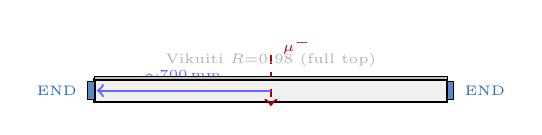
\begin{tikzpicture}[scale=0.56, every node/.style={font=\tiny}]
  \draw[thick,fill=gray!12] (0,0) rectangle (8,0.5);
  \draw[fill=bluecol!80] (-0.15,0.05) rectangle (0,0.45);
  \draw[fill=bluecol!80] (8.00,0.05) rectangle (8.15,0.45);
  \draw[->,thick,red!70!black,dashed] (4.0,1.05) -- (4.0,-0.1);
  \node[above right,text=red!70!black] at (4.05,0.85) {$\mu^-$};
  \draw[->,blue!60,thick] (4.0,0.25) -- (0.05,0.25);
  \node[above,text=blue!60] at (2.0,0.28) {$\sim$700\,mm};
  \draw[fill=gray!50] (0,0.5) rectangle (8.0,0.57);
  \node[above,text=gray!60] at (4.0,0.57) {Vikuiti $R{=}0.98$ (full top)};
  \node[left,text=bluecol] at (-0.18,0.25) {END};
  \node[right,text=bluecol] at (8.18,0.25) {END};
\end{tikzpicture}
\end{center}

\vspace{0.2em}
Photons travel $\sim$700\,mm before detection.
\vspace{0.2em}

\footnotesize
\begin{tabular}{ll}
\toprule
Effect & Impact\\
\midrule
Long propagation & large time spread\\
Multiple reflections & Vikuiti losses\\
$\tau_{\rm prop}\sim3.7$\,ns & propagation-limited\\
\bottomrule
\end{tabular}\\[0.3em]
$\Rightarrow$ $\sE = 50.5$\,ps \ (best with $m^*{=}7$)
\end{column}

\begin{column}{0.47\textwidth}
\textbf{EndSparseTop (new):}\\[0.3em]
\begin{center}
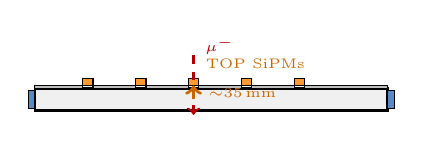
\begin{tikzpicture}[scale=0.56, every node/.style={font=\tiny}]
  \draw[thick,fill=gray!12] (0,0) rectangle (8,0.5);
  \draw[fill=bluecol!80] (-0.15,0.05) rectangle (0,0.45);
  \draw[fill=bluecol!80] (8.00,0.05) rectangle (8.15,0.45);
  \foreach \xi in {1.2,2.4,3.6,4.8,6.0}
    \draw[fill=orange!80] (\xi-0.12,0.57) rectangle (\xi+0.12,0.72);
  \draw[fill=gray!50] (0,0.50) rectangle (1.08,0.57);
  \draw[fill=gray!50] (1.32,0.50) rectangle (2.28,0.57);
  \draw[fill=gray!50] (2.52,0.50) rectangle (3.48,0.57);
  \draw[fill=gray!50] (3.72,0.50) rectangle (4.68,0.57);
  \draw[fill=gray!50] (4.92,0.50) rectangle (5.88,0.57);
  \draw[fill=gray!50] (6.12,0.50) rectangle (8.0,0.57);
  \draw[->,thick,red!70!black,dashed] (3.6,1.25) -- (3.6,-0.1);
  \node[above right,text=red!70!black] at (3.65,1.05) {$\mu^-$};
  \draw[->,orange!80!black,very thick] (3.6,0.25) -- (3.6,0.57);
  \node[right,text=orange!80!black] at (3.72,0.40) {$\sim$35\,mm};
  \node[above,text=orange!80!black] at (5.0,0.72) {TOP SiPMs};
\end{tikzpicture}
\end{center}

\vspace{0.2em}
TOP SiPMs capture photons after only $\sim$35\,mm.
\vspace{0.2em}

\footnotesize
\begin{tabular}{lcc}
\toprule
 & END & TOP ($N{=}20$)\\
\midrule
Path & $\sim$700\,mm & $\sim$35\,mm\\
$\tau_{\rm prop}$ & $\sim$3.7\,ns & $\sim$185\,ps\\
Limit & propagation & scintill.\ $\tau$\\
$\sigma$ measured & 53.7\,ps & \textbf{15.2\,ps}\\
\bottomrule
\end{tabular}\\[0.3em]
$\Rightarrow$ Near-field: short, uniform photon paths.
\end{column}
\end{columns}
\end{frame}

% ── 3. ESTIMATORS ─────────────────────────────────────────────────────────────
\begin{frame}{How the estimators are built}
\begin{columns}[T]
\begin{column}{0.48\textwidth}
\textbf{END: $m$-average}\\[0.3em]
\footnotesize
Sort photon times on left (L) and right (R) ends.
Take mean of first $m$ times on each side:
\normalsize
\[
T_0^{\rm END}(m) = \frac{\overline{t_L^{1\ldots m}} + \overline{t_R^{1\ldots m}}}{2}
\]
\footnotesize
Averaging reduces noise; too large $m$ mixes in late photons. Optimal $m^*$.\\[0.3em]
\textbf{Verified:} $m^* = 8$, \ $\sE = 53.68\pm0.93$\,ps

\vspace{0.5em}
\normalsize
\textbf{TOP: $k$-th order statistic}\\[0.3em]
\footnotesize
Pool all arrival times on top face (all $N$ SiPMs).
Take the $k$-th earliest:
\normalsize
\[
T_0^{\rm TOP}(k) = t_{\rm TOP}^{(k)}
\]
\footnotesize
$k{=}1$: maximum fluctuation from isolated early photons.
$k{=}2$--$3$: plateau — noise reduced. Large $k$: longer paths included.\\[0.3em]
\textbf{Verified:} $k^* = 3$, \ $\sT = 15.20\pm0.27$\,ps
\end{column}

\begin{column}{0.48\textwidth}
\textbf{BLUE combination}\\[0.3em]
\footnotesize
Combine $T_0^{\rm END}$ and $T_0^{\rm TOP}$ with optimal weights:
\normalsize
\[
T_0^{\rm BLUE} = w_E\,T_0^{\rm END} + w_T\,T_0^{\rm TOP}
\]
\[
w_E = \frac{\sigma_T^2 - \mathrm{cov}}{\sigma_E^2 + \sigma_T^2 - 2\,\mathrm{cov}}
\]
\footnotesize
Covariance measured event-by-event.

\vspace{0.4em}
\renewcommand{\arraystretch}{1.2}
\begin{tabular}{lr}
\toprule
Quantity & Value\\
\midrule
$\sE$ & $53.7\pm0.9$\,ps\\
$\sT$ & $15.20\pm0.27$\,ps\\
$\rho(T_{\rm END},T_{\rm TOP})$ & $0.16$\\
$w_{\rm END}$ & $\WEND$\\
$w_{\rm TOP}$ & $\WTOP$\\
\midrule
$\sB$ (event-by-event) & $15.21\pm0.26$\,ps\\
$\sB$ (from covariance) & $15.18$\,ps\ \checkmark\\
\bottomrule
\end{tabular}

\vspace{0.4em}
Cross-check passed: $\sigma_{\rm BLUE}^{\rm cov}=15.18$ vs $\sigma_{\rm BLUE}^{\rm ev}=15.21$\,ps.\\[0.3em]
$w_{\rm TOP}\approx 1$ \ $\Rightarrow$ BLUE $\approx$ TOP alone.\\[0.2em]
\textit{Resolution: $\sigma_{\rm IQR}=(Q_{75}-Q_{25})/1.349$.}
\end{column}
\end{columns}
\end{frame}

% ── 4. FINDING THE OPTIMUM ────────────────────────────────────────────────────
\begin{frame}{Finding the optimal estimator}
\begin{columns}[T]
\begin{column}{0.51\textwidth}

\includegraphics[width=\textwidth,height=5.2cm,keepaspectratio]{\plots/fig1_kscan.png}
\end{column}

\begin{column}{0.45\textwidth}
\footnotesize
\textbf{$k$-scan, TOP} (EJ-230, $N{=}20$, $x{=}0$):
\vspace{0.1em}

\begin{itemize}\setlength{\itemsep}{0pt}
  \item $k{=}1$: earliest photon — large fluctuation
  \item $k{=}2$--$3$: minimum — noise reduced
  \item $k{>}5$: $\sigma$ rises — longer paths enter
  \item[$\Rightarrow$] $k^* = 3$, \ $\sT = 15.20\pm0.27$\,ps
\end{itemize}

\vspace{0.2em}
\normalsize\textbf{All $N$ (EJ-230, $x{=}0$):}\vspace{0.1em}

\footnotesize
\renewcommand{\arraystretch}{1.1}
\begin{tabular}{ccccc}
\toprule
$N$ & Total & $m^*$ & $k^*$ & $\sT$\,[ps]\\
\midrule
4  & 20 & 12 & 1 & $78.2\pm1.8$\\
8  & 24 &  9 & 1 & $32.0\pm0.6$\\
14 & 30 &  9 & 2 & $18.7\pm0.3$\\
\rowcolor{rowbest}
20 & 36 &  8 & 3 & $\mathbf{15.20\pm0.27}$\\
\bottomrule
\end{tabular}

\vspace{0.2em}
Higher $N$ $\Rightarrow$ more near-field photons $\Rightarrow$ larger $k^*$.
\end{column}
\end{columns}
\end{frame}

% ── 5. THE 15 ps RESULT ───────────────────────────────────────────────────────
\begin{frame}{The 15\,ps result — residual distributions}
\begin{columns}[T]
\begin{column}{0.52\textwidth}

\includegraphics[width=\textwidth,height=5.2cm,keepaspectratio]{\plots/fig2_residuals.png}
\end{column}

\begin{column}{0.44\textwidth}
\footnotesize
\textbf{EJ-230, $N{=}20$, $x{=}0$, 5000 events}

\vspace{0.15em}
\renewcommand{\arraystretch}{1.1}
\begin{tabular}{lrr}
\toprule
 & $\sigma_{\rm IQR}$ & $\sigma_{\rm Gauss}$\\
\midrule
END ($m^*{=}8$) & $53.7$\,ps & $53.3$\,ps\\
TOP ($k^*{=}3$) & $15.20$\,ps & $14.93$\,ps\\
\rowcolor{rowbest}
BLUE & $\mathbf{15.21}$\,ps & $14.80$\,ps\\
\bottomrule
\end{tabular}

\vspace{0.2em}
\begin{itemize}\setlength{\itemsep}{0pt}
  \item END: Gaussian OK ($p{=}0.09$); $\sigma_{\rm IQR}\approx\sigma_G$.
  \item TOP/BLUE: non-Gaussian tails; IQR is official metric.
  \item BLUE $\approx$ TOP: $w_{\rm TOP}{=}0.987$; END negligible.
\end{itemize}

\vspace{0.2em}
\textit{Timing comes almost entirely from TOP.}
\end{column}
\end{columns}
\end{frame}

% ── 6. WHY DOES IT WORK? ──────────────────────────────────────────────────────
\begin{frame}{Why does it work? Near-field photon statistics}
\begin{columns}[T]
\begin{column}{0.49\textwidth}
\textbf{Photon yield (EJ-230, $x{=}0$):}\\[0.2em]
\footnotesize
\renewcommand{\arraystretch}{1.15}
\begin{tabular}{lcc}
\toprule
Face & $N_{\rm pe}$/ev & $\sigma$\\
\midrule
LEFT end  & 514.9 & $\sim$54\,ps\\
RIGHT end & 515.0 & $\sim$54\,ps\\
\rowcolor{rowbest}
TOP ($N{=}20$) & 1341 & \textbf{15.2\,ps}\\
\bottomrule
\end{tabular}

\vspace{0.5em}
\normalsize
\textbf{Scale estimate (near-field limit):}
\[
\sigma \sim \frac{\tau_{\rm rise}}{\sqrt{N_{\rm pe}}}
\quad\xrightarrow{{\rm EJ\text{-}230}}\quad
\frac{500\,{\rm ps}}{\sqrt{1341}} = 13.7\,{\rm ps}
\]
\footnotesize
Measured: $15.2$\,ps — consistent.\\[0.2em]
\textit{Sanity check only; $k^*$ estimator uses order statistics, not a full average.}
\end{column}

\begin{column}{0.47\textwidth}
\textbf{Nearest SiPM distance vs regime:}\\[0.2em]
\footnotesize
$n{=}1.58$, \ $v{=}c/n{=}190\,{\rm mm/ns}$

\vspace{0.2em}
\renewcommand{\arraystretch}{1.2}
\setlength{\tabcolsep}{5pt}
\begin{tabular}{crrl}
\toprule
$N$ & $d_{\rm max}$ & $\tau_{\rm prop}$ & Regime\\
\midrule
4  & 175\,mm & 920\,ps & $\tau_p \gg \tau_r$\\
8  & 87.5\,mm & 460\,ps & $\tau_p \approx \tau_r$\\
14 &  50\,mm & 263\,ps & $\tau_p \sim \tau_r$\\
\rowcolor{rowbest}
20 &  35\,mm & \textbf{184\,ps} & $\tau_p < \tau_r$\\
\bottomrule
\end{tabular}

\vspace{0.3em}
\normalsize
$\tau_r = \tau_{\rm rise} = 500$\,ps for EJ-230.

\vspace{0.4em}
At $N{=}20$: propagation time $<$ rise time
$\Rightarrow$ near-field regime.

\vspace{0.4em}
\footnotesize
For $N{=}4$ (nearest SiPM at 175\,mm): propagation
dominates and the $\tau/\sqrt{N_{\rm pe}}$ model fails.
$N{\geq}14$ approaches the scintillation limit.
\end{column}
\end{columns}
\end{frame}

% ── 7. POSITION DEPENDENCE ────────────────────────────────────────────────────
\begin{frame}{Position dependence — $N{=}20$, EJ-230}
\begin{columns}[T]
\begin{column}{0.52\textwidth}

\includegraphics[width=\textwidth,height=5.2cm,keepaspectratio]{\plots/fig3_sigma_vs_x.png}
\end{column}

\begin{column}{0.44\textwidth}
\footnotesize
\textbf{Fit and range (13 positions):}
\vspace{0.1em}

\renewcommand{\arraystretch}{1.1}
\begin{tabular}{ll}
\toprule
Min $\sB$ & $14.6\pm0.3$\,ps ($x{=}-100$\,mm)\\
Max $\sB$ & $17.8\pm0.3$\,ps ($x{=}+200$\,mm)\\
Peak-to-peak & $3.2$\,ps (21\%)\\
\midrule
Const.\ fit $C$ & $15.75\pm0.08$\,ps\\
$\chi^2$/ndf & $163/12$\\
$p$-value & $<0.001$\\
\bottomrule
\end{tabular}

\vspace{0.2em}
\normalsize\textbf{Interpretation:}\vspace{0.1em}
\footnotesize
\begin{itemize}\setlength{\itemsep}{0pt}
  \item Variation \textbf{statistically real} ($\chi^2/{\rm ndf}=163/12$).
  \item Near SiPM ($\leq$5\,mm): $\sigma\approx14.6$--$15$\,ps;\\
        at gap midpoint ($\sim$25\,mm): $\sigma\approx17$--$18$\,ps.
  \item \textbf{3--4$\times$ better than END+Vik} everywhere.
  \item Engineering: approx.\ uniform; NOT statistically flat.
\end{itemize}
\end{column}
\end{columns}
\end{frame}

% ── 8. BLUE WEIGHTS ───────────────────────────────────────────────────────────
\begin{frame}{BLUE weights: what does END actually contribute?}
\begin{columns}[T]
\begin{column}{0.53\textwidth}
\vspace{0.2em}
\scriptsize
\setlength{\tabcolsep}{4pt}
\renewcommand{\arraystretch}{1.35}
\begin{tabular}{crrrrrr}
\toprule
$N$ & $\sE$\,[ps] & $\sT$\,[ps] & $\rho$ & $w_E$ & $w_T$ & $\sB$\,[ps]\\
\midrule
4  & 51.0 & 78.2 & 0.15 & 0.74 & 0.26 & $45.5\pm0.8$\\
8  & 50.2 & 32.0 & 0.18 & 0.21 & 0.79 & $28.9\pm0.5$\\
14 & 51.0 & 18.7 & 0.18 & 0.02 & 0.98 & $18.2\pm0.3$\\
\rowcolor{rowbest}
20 & 53.7 & 15.2 & 0.16 & 0.013 & 0.987 & $\mathbf{15.2\pm0.3}$\\
\bottomrule
\end{tabular}

\vspace{0.4em}
\footnotesize
\textbf{Correlation $\rho\approx0.16$:} low but non-zero.
TOP SiPMs absorb some photons that would otherwise
reach the END SiPMs — weak anticorrelation of yields.

\vspace{0.3em}
\textbf{BLUE cross-check ($N{=}20$):}\\
$\sigma_{\rm BLUE}^{\rm event}=15.21$\,ps vs
$\sigma_{\rm BLUE}^{\rm cov}=15.18$\,ps \ \checkmark\\[0.2em]
\textit{No bug. BLUE implementation correct.}
\end{column}

\begin{column}{0.43\textwidth}
\vspace{0.2em}
\footnotesize
\textbf{Weight distribution at $N{=}20$:}

\vspace{0.3em}
\begin{center}
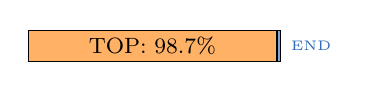
\begin{tikzpicture}[scale=0.80]
  \draw[fill=orange!60] (0,0) rectangle (3.95,0.5);
  \draw[fill=bluecol!60] (3.95,0) rectangle (4.0,0.5);
  \node at (1.97,0.25) {\footnotesize TOP: 98.7\%};
  \node[right,font=\tiny,bluecol] at (4.02,0.25) {END};
\end{tikzpicture}
\end{center}

\vspace{0.4em}
\normalsize
\textbf{Key conclusion:}

\vspace{0.2em}
\begin{center}
\fbox{\parbox{0.88\linewidth}{\centering\footnotesize
The improvement from 50\,ps to 15\,ps\\
is driven \textbf{entirely by the TOP SiPMs}.\\[0.2em]
The 16 END SiPMs carry $<\!1.3\%$\\
of the BLUE weight at $N_{\rm top}{=}20$.
}}
\end{center}

\vspace{0.4em}
\footnotesize
$\Rightarrow$ \textbf{Next step:} reduce END SiPMs\\
(e.g.\ 4 per face instead of 8) while\\
keeping $N_{\rm top}{=}20$.\\
Expected $\sigma$ penalty: small.
\end{column}
\end{columns}
\end{frame}

% ── 9. σ vs N_top ─────────────────────────────────────────────────────────────
\begin{frame}{$\sigma$ vs number of TOP SiPMs}
\begin{columns}[T]
\begin{column}{0.62\textwidth}

\includegraphics[width=\textwidth,height=5.5cm,keepaspectratio]{\plots/fig4_sigma_vs_ntop.png}
\end{column}

\begin{column}{0.34\textwidth}
\scriptsize
\textbf{Left panel:}\\
$\sigma_{\rm TOP}$ and $\sigma_{\rm BLUE}$ vs $N_{\rm top}$.\\
END+Vik ref (50.5\,ps) dashed.\\
$\sigma_{\rm BLUE}\approx\sigma_{\rm TOP}$ for $N{\geq}14$.

\vspace{0.2em}
\textbf{Right panel:}\\
$\sigma_{\rm TOP}$ vs nearest SiPM distance.\\
$\tau_p{=}d/v_{\rm sc}$ shown as dashed guide.\\
$N{=}4$ ($d{=}175$\,mm): propagation\\
dominates; $\tau/\sqrt{N_{\rm pe}}$ model fails.\\
$N{\geq}14$: $\tau_p{<}\tau_{\rm rise}$, scintil.\ limit.

\vspace{0.2em}
\textbf{Diminishing returns:}\\
$N{:}\ 8{\to}14$: $-11$\,ps\\
$N{:}\ 14{\to}20$: $-3.5$\,ps
\end{column}
\end{columns}
\end{frame}

% ── 10. EJ-204 vs EJ-230 ─────────────────────────────────────────────────────
\begin{frame}{EJ-230 vs EJ-204: are they really different?}
\begin{columns}[T]
\begin{column}{0.50\textwidth}
\footnotesize
\renewcommand{\arraystretch}{1.3}
\begin{tabular}{lrrr}
\toprule
Config & $\sigma_{\rm BLUE}$ & Uncertainty & $N_{\rm pe}^{\rm TOP}$\\
\midrule
EJ-230, $N{=}20$ & 15.21\,ps & $\pm0.26$\,ps & 1341\\
EJ-204, $N{=}20$ & 15.14\,ps & $\pm0.28$\,ps & 1615\\
\midrule
Difference & \multicolumn{3}{l}{$-0.07\pm0.38$\,ps \quad $(0.2\,\sigma)$}\\
\bottomrule
\end{tabular}

\vspace{0.5em}
\begin{center}
\normalsize\textbf{EJ-204 and EJ-230 are statistically\\equivalent at $N_{\rm top}{=}20$.}
\end{center}

\vspace{0.3em}
\footnotesize
No evidence for a real timing difference.
EJ-204 has more top photons (1615 vs 1341),
but the $k^*$-order-statistic already captures
the minimum-time behaviour; extra photons
give diminishing returns.
\end{column}

\begin{column}{0.46\textwidth}
\footnotesize
\textbf{Why was EJ-230 recommended?}\\[0.3em]
\begin{enumerate}
  \item \textbf{Phase I}: EJ-230 better in END-only mode\\
        (50.5 vs 53.4\,ps with $m^*$ estimator).
  \item \textbf{Speed}: $\tau{=}1.5$\,ns vs $1.8$\,ns\\
        — faster emission, benefits other regimes.
  \item \textbf{Attenuation}: $L_{\rm att}{=}120$\,cm vs $160$\,cm\\
        — less re-absorption at far end.
  \item \textbf{Phase II}: No preference at $N{=}20$.\\
        Both give $15.1$--$15.2$\,ps.
\end{enumerate}

\vspace{0.4em}
\normalsize
\textbf{Recommendation:}\\
\footnotesize
Either scintillator is acceptable for EST $N{=}20$.
Choose on cost, availability, non-timing criteria.
Do \textbf{not} claim EJ-230 is timing-superior here.
\end{column}
\end{columns}
\end{frame}

% ── CONCLUSIONS ───────────────────────────────────────────────────────────────
\begin{frame}{Conclusions}
\begin{columns}[T]
\begin{column}{0.50\textwidth}
\footnotesize
\textbf{Verified results (EJ-230, all from ROOT files):}

\vspace{0.3em}
\renewcommand{\arraystretch}{1.25}
\begin{tabular}{lr}
\toprule
END+Vikuiti reference & $50.5$\,ps\\
\midrule
\rowcolor{rownew}
EST $N{=}4$, BLUE  & $45.5\pm0.8$\,ps\\
\rowcolor{rownew}
EST $N{=}8$, BLUE  & $28.9\pm0.5$\,ps\\
\rowcolor{rownew}
EST $N{=}14$, BLUE & $18.2\pm0.3$\,ps\\
\rowcolor{rowbest}
EST $N{=}20$, BLUE & $\mathbf{15.21\pm0.26}$\,ps\\
\bottomrule
\end{tabular}

\vspace{0.4em}
\textbf{Position uniformity ($N{=}20$):}\\
Range $14.6$--$17.8$\,ps; $3.2$\,ps peak-to-peak.\\
Variation is real, correlates with SiPM spacing.\\
"Approximately uniform" — not statistically flat.\\[0.3em]
\textbf{EJ-204 $\approx$ EJ-230:} diff $0.07\pm0.38$\,ps ($0.2\,\sigma$).
\end{column}

\begin{column}{0.46\textwidth}
\footnotesize
\textbf{Four key messages:}\\[0.3em]
\begin{enumerate}
  \item \textbf{TOP SiPMs drive the improvement}\\
        Near-field ($\sim$35\,mm) vs far-field ($\sim$700\,mm).\\
        Factor $3.3\times$ better than END+Vik.

  \vspace{0.2em}
  \item \textbf{EJ-204 and EJ-230 are equivalent}\\
        at $N{=}20$. No timing preference.

  \vspace{0.2em}
  \item \textbf{END SiPMs contribute $<$1.3\% of BLUE weight}\\
        at $N{=}20$. Timing is almost entirely\\
        determined by the TOP measurement.

  \vspace{0.2em}
  \item \textbf{Next: reduce END SiPMs}\\
        Explore 4 per face instead of 8.\\
        Expected $\sigma$ impact: negligible.
\end{enumerate}
\end{column}
\end{columns}
\end{frame}

\end{document}
